\documentclass[a4paper,11pt]{article}
\usepackage[utf8]{inputenc}
\usepackage[english]{babel}
\usepackage{amssymb}
\usepackage{amsmath}
\usepackage{amsthm}
\usepackage{mathrsfs}
\usepackage{array}
\usepackage{graphicx}
\usepackage[usenames,dvipsnames]{color}
\usepackage{listings}
\usepackage{arydshln}
\usepackage{multirow}
%\usepackage{slashbox}
\usepackage{subfigure}
\usepackage{pdflscape}
%\usepackage{cancel}
%\usepackage[bookmarks = false]{hyperref}
\usepackage[left=1.75cm, right=1.75cm, top=2cm, bottom=2cm]{geometry}

\newcommand{\ttsee}[1]{Voir \texttt{#1}\paragraph{}}
\newcommand{\ttseek}[1]{Voir package \texttt{#1}\paragraph{}}


% Initialisation de listings
%\definecolor{mymauve}{rgb}{0.63,0.13,0.94}
%\definecolor{mygreen}{rgb}{0.13,0.55,0.13}
%\definecolor{mybeige}{rgb}{0.99,0.99,0.86}
%\definecolor{mygris}{rgb}{0.8,0.8,0.8}
\definecolor{light-gray}{gray}{0.50}
\lstset{
    columns=flexible,
	%numbers = left,				% placement de la numérotation des lignes
	numberstyle = \small,        	% taille du numéro de ligne
	stepnumber = 1,              	% ???
	numbersep = 10pt,            	% taille de l'espace de séparation entre numéro de ligne et code
	showspaces = false,          	% montrer les espaces
	showstringspaces=false,         % enlever les espaces str
	showtabs = false,            	% montrer les tabulations
	tab = rightarrowfill,        	% ???
	tabsize=3,						% tabulation size
	language = Java,             	% langage utilisé
	basicstyle = \footnotesize\tt,	% ???
	captionpos = b,					% ???
	linewidth=\linewidth,			% largeur de la fenetre de code
	breaklines = true,				% ???
	commentstyle = \color{light-gray}, % définition de la couleur des commentaires
	%stringstyle = \color{mymauve},  % définition de la couleur des chaines de caractères
	%identifierstyle = \ttfamily,    % ???
	keywordstyle = \color{blue},	% définition de la couleur des mots clés
	%frame=single,
	%backgroundcolor=\color{mybeige},
	extendedchars=true				% étend les caractères pouvant être utilisés
}

%\author{Mormont Romain}
%\title{Synthèse : Base de données (Pierre Wolper)}
%\date{Année académique 2013-2014}

\begin{document}
\rule{1\linewidth}{1px}
{ \sc
\begin{center}
{\small University of Liège}\\
{\small Faculty of Applied Sciences}

\end{center}

\vfill
\begin{center}

{\Huge Object Oriented Software Engineering {\LARGE \tt [INFO0063]}\\}
\end{center}
\begin{center}
{\Huge Project : Report}
\end{center}
\begin{center}
\textbf{Magera Floriane}\\
{\small 1$^{\text{st}}$ master in computer engineering}\\
{\small Option : Computer systems and networks}\\
{\small s111295}\\
\vspace{0.5cm}
\textbf{Servais Fabrice}\\
{\small 1$^{\text{st}}$ master in computer engineering}\\
{\small Option : Computer systems and networks}\\
{\small s111093}\\
\vspace{0.5cm}
\textbf{Mormont Romain}\\
{\small 1$^{\text{st}}$ master in computer engineering}\\
{\small Option : Intelligent systems}\\
{\small s110940}
\end{center}

\vfill
\begin{center}
Academic year 2014-2015\\
\end{center}
}
\rule{1\linewidth}{1px}
\newpage
\tableofcontents
\newpage

\section{Introduction}

This report presents the solution we have developed for the INFO0063 course project. In the Section \ref{sec:diagrams}, we will first discuss about the diagrams we have chosen for describing the concept and design of the application. In the Section \ref{sec:patterns}, we will present the patterns we have included in our solution and, finally, in the Section \ref{sec:cls_hier}, we will say few words about our class hierarchy.

\section{Diagrams}
\label{sec:diagrams}
	
	\subsection{Conceptual}

At the conceptual level, we provide 2 diagrams of different kinds to show the whole program : class and activity diagrams.

\paragraph{}

The conceptual class diagram is shown \textsc{Figure} \ref{fig:concept-class}. It shows the main classes that compose the game : \texttt{Logic} and \texttt{GUI}. The GUI have some basic components which show briefly what the users will see, and some methods explaining the role of the GUI (which is displaying information). The logic keeps the information concerning the state of the game, at a higher level in this diagram. Here, \texttt{Logic} is acting like as an interface between the state and the GUI. We can also see that the state of game is composed of a \texttt{Board} containing \texttt{Cell}'s of different kind. Methods are also provided to change and update the state of the game.

\paragraph{}

The conceptual activity diagram is shown \textsc{Figure} \ref{fig:concept-activity} and \ref{fig:concept-generate-board}. It represents the proceedings of the program during a game. The first part concerns the creation of the board, it is shown on the sub-activity diagram \textsc{Figure} \ref{fig:concept-generate-board}. The file is simply parsed in order to create \texttt{Cell}'s to create a \texttt{Board}. The rest of the main diagram shows the reaction following an action of the user : 
\begin{itemize}
	\item Click on a cell : the board is recomputed and one checks if it is a winning move.
	\item Click on the undo button : cancel the last action.
	\item Click on the reset button : restart from the beginning.
	\item Quit : simply close the program.
\end{itemize}


\subsection{Design}
We have chosen sequence and class diagrams to document our application design. 
\subsubsection{Interfaces}
The interfaces are given in the diagram in Figure \ref{fig:inter}.
\subsubsection{Logic}
The logic core class is the \texttt{Logic} class which implements the logic interface and is thus the main entry point of the logic subsystem. This class interacts with the following :
\begin{itemize}
	\item reversible actions : classes \texttt{Stack<Command>}, \texttt{Command} and \texttt{Rotation} 
	\item game board : classes \texttt{Board} and \texttt{Cell}
	\item configuration file parsing : class \texttt{Parser}
	\item chronometer : class \texttt{PeriodicNotifier}
\end{itemize}
These components are described in the diagram of Figure \ref{fig:logic}.
\subsubsection{Cells}
Cells are the other possible entry point of the logic subsystem as it implements the cell interface. The cells and related classes are described in the diagram of Figure \ref{fig:cells}.
\subsubsection{Algorithms and data structures}
We have decided to document the following actions/algorithms with diagrams :
\begin{itemize}
	\item Handling of the rotation requests issued by the GUI through \texttt{Logic.rotate(int i, int j)}, \texttt{Cell.clockwiseNext()} or \texttt{Cell.counterClockwiseNext()} : see Figure \ref{fig:rot_request}
	\item Execution of the rotation operation : see Figure \ref{fig:rotation}.
	\item Handling and execution of the undo operation  : see Figure \ref{fig:undo}
	\item Handling and execution of the reset operation : see Figure \ref{fig:reset}
	\item Update of the supply state of each cell of the board : see Figure \ref{fig:sup_update}
\end{itemize}
\section{Applied patterns}
\subsection{Observer}
The observer pattern is applied two times : 
\begin{enumerate}
	\item The logic is observed by the UI through the common interface (interfaces \texttt{Observable} and \texttt{Observer})
	\item The cells are observed by the Logic
\end{enumerate}
The first application of the pattern allows the UI to update its state when logic updates its own leading to more independence between the subsystems. We have : 
\begin{itemize}
	\item \textit{AbstractObserver} : \texttt{Observer}
	\item \textit{AbstractSubject} : \texttt{Observable}
	\item \textit{ConcreteObserver} : \texttt{GUI}
	\item \textit{ConcreteSubject} : \texttt{Logic}
\end{itemize}
\paragraph{}
 This structure implies that the class that implements \texttt{LogicInterface} must be aware of any modification of the logic subsystem state in order to generate proper notification to the GUI. The structure of the interface is such that it is not always the case. Indeed, the \texttt{CellInterface} provides two methods for rotating the cells and thus changing the logic state. The UI can thus bypasses the \texttt{Logic} class which cannot be aware of this state modification and cannot trigger the update notification to the UI.
\\ \\ 
We thus have to develop a mechanism so that any cell is able to notify the logic that it receives a rotation request. To do so, we use the observer pattern again :
\begin{itemize}
	\item \textit{AbstractObserver} : \texttt{RotationRequestObserver}
	\item \textit{AbstractSubject} : \texttt{RotationRequestNotifier}
	\item \textit{ConcreteObserver} : \texttt{Logic}
	\item \textit{ConcreteSubject} : \texttt{Cell}
\end{itemize}
\paragraph{}
The cells are observed by the logic main class and communicates its coordinates and the rotation direction through the notify call. The logic class can then execute the rotation and notifies the UI of the modification.
\subsection{Command}
The interactions between the logic and the UI can be summarized into three types of request : undo, reset and rotate.  The undo and reset operations are directly implemented in the methods of the \texttt{Logic} class. The rotate operation is a little more complicated because it should be reversible when the user wants to undo one of its move. The idea is thus to encapsulate this operation and its reverse into an object : this is the \textbf{command} pattern. In this case, there is a slight variation compared the pattern explained during the lecture. Indeed, the \textit{Invoker} and the \textit{Client} are the same class : 
\begin{itemize}
	\item \textit{Client}, \textit{Invoker} : \texttt{Logic}
	\item \textit{Command} : \texttt{Command}
	\item \textit{ConcreteCommand} : \texttt{Rotation}
	\item \textit{Receiver} : \texttt{Board}
\end{itemize}
\paragraph{}
The command interface thus specifies two methods for executing and reversing the operation : \texttt{execute()} and \texttt{reverse()}. The advantage of this method is that extending the set of reversible operations is very easy and the implementation of the \texttt{undo} is independent of the actual action of the operation to reverse. 
\subsection{Builder and singleton}
The cells are relatively complex to build because they need to be fed with coordinates, a Piece enumeration value, an Orientation enumeration value, an observer,... To avoid duplicating the object construction logic over many location in the code, we have created a \texttt{CellBuilder} object which is responsible for creating the cells. Also, it is not necessary to have duplicate instance of this object. Therefore, we have used the singleton pattern for this class.
\label{sec:patterns}
\section{Class hierarchy}
\label{sec:cls_hier}
\section{Conclusion}
\appendix
\section{Conceptual}
\subsection{Class diagrams}
\begin{figure}[h]
	\center
	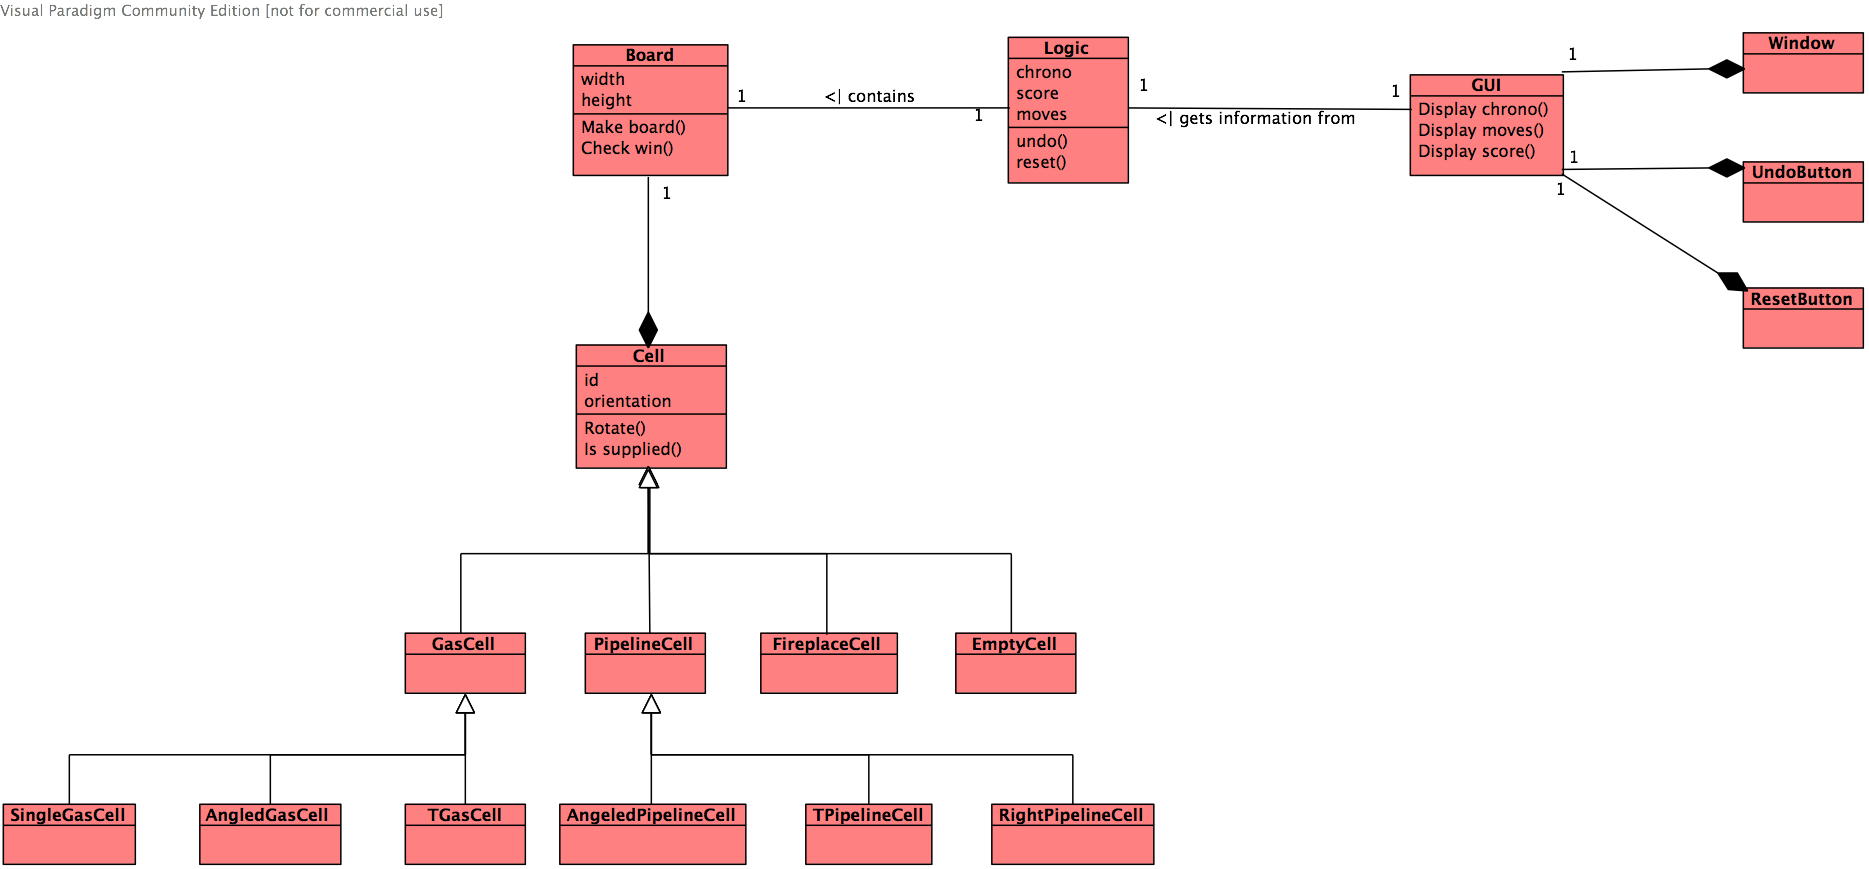
\includegraphics[angle=90,scale=0.8]{Conceptual-Class-diagram.png}
	\caption{Conceptual class diagram}
	\label{fig:concept-class}
\end{figure}

\subsection{Activity diagram}
\begin{figure}[h]
	\center
	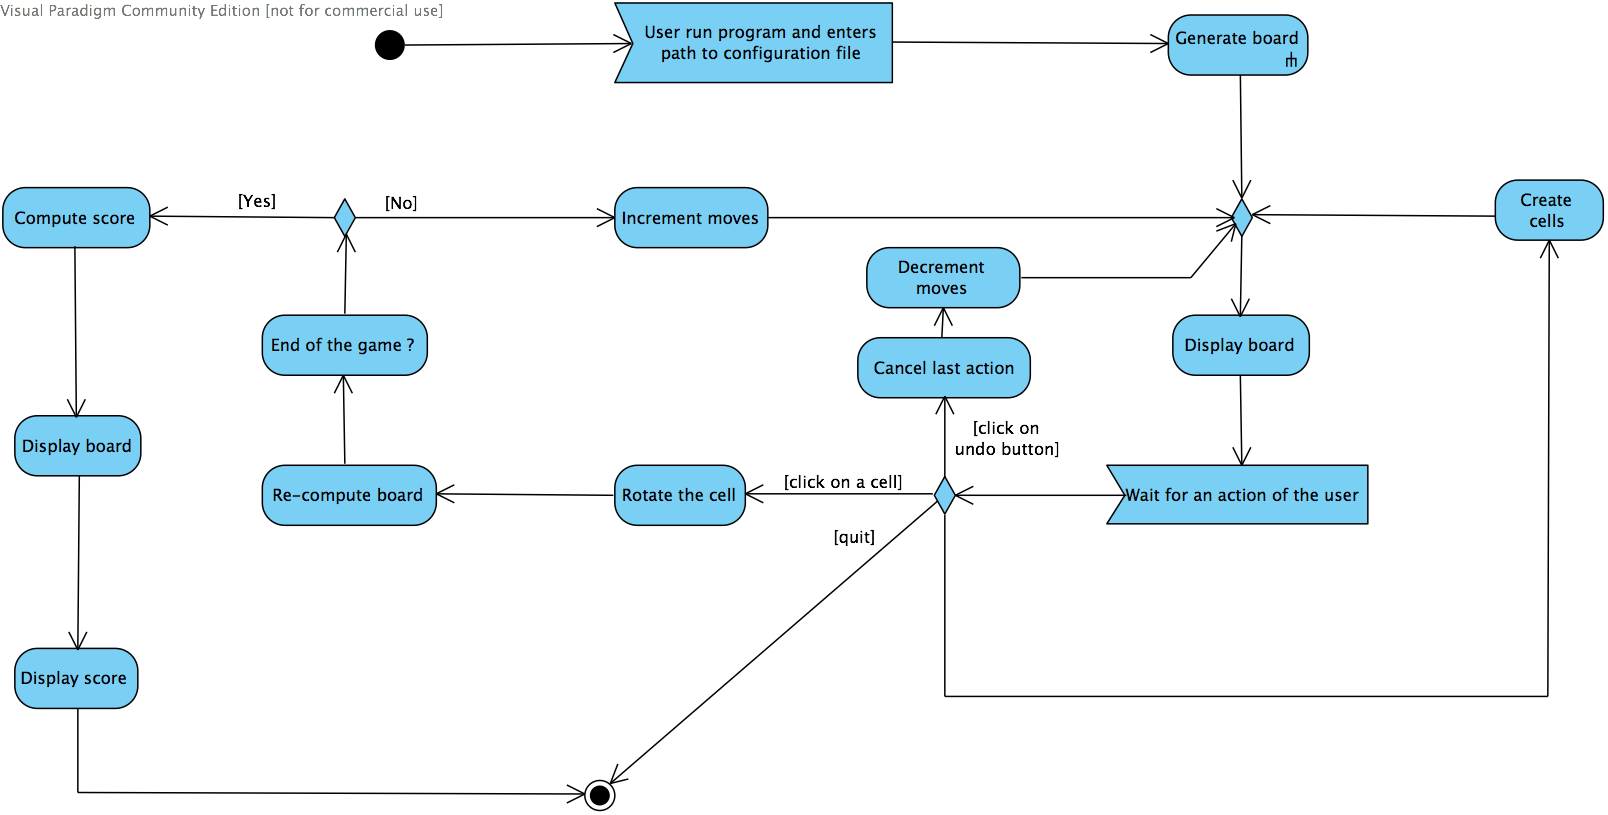
\includegraphics[angle=90,scale=0.9]{Conceptual-activity-diagram.png}
	\caption{Conceptual activity diagram - Game}
	\label{fig:concept-activity}
\end{figure}

\begin{figure}[h]
	\center
	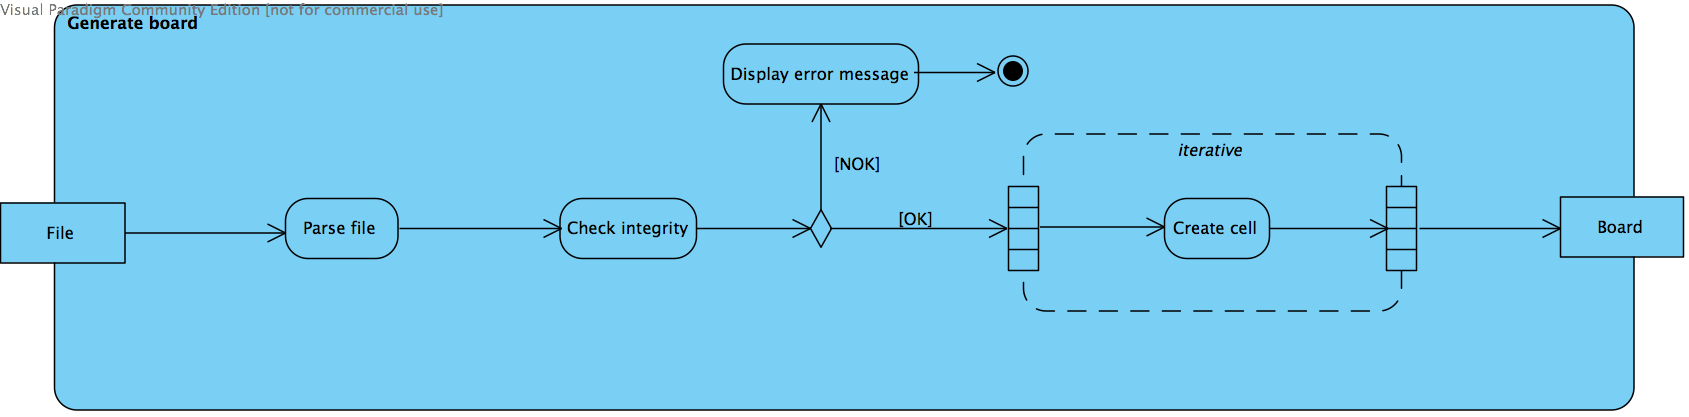
\includegraphics[angle=90,scale=0.7]{Generate-board.png}
	\caption{Conceptual sub-activity diagram - Generate board}
	\label{fig:concept-generate-board}
\end{figure}

\section{Design}
\subsection{Class diagrams}
\begin{figure}[h]
	\center
	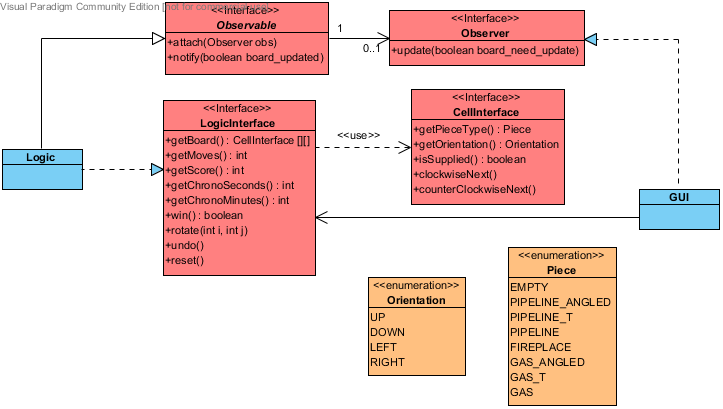
\includegraphics[angle=90,scale=1]{interfaces.png}
	\caption{Interfaces}
	\label{fig:inter}
\end{figure}
\begin{figure}[h]
	\center
	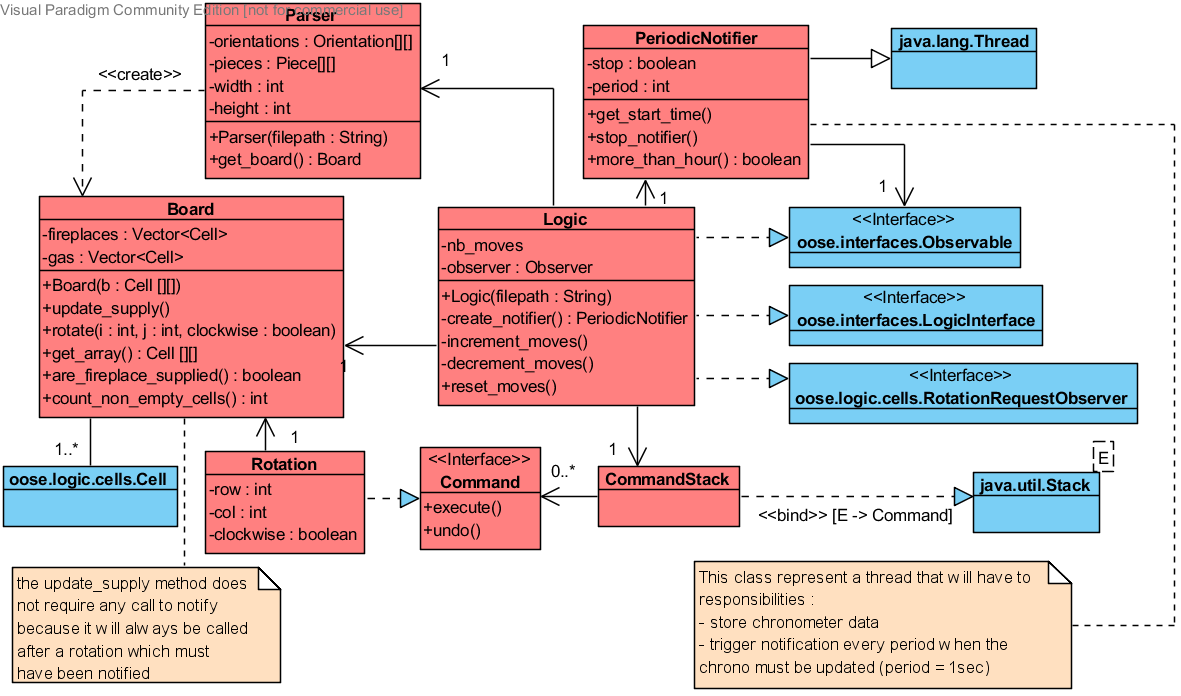
\includegraphics[angle=90,scale=1]{logic.png}
	\caption{Logic core}
	\label{fig:logic}
\end{figure}
\begin{figure}
	\center
	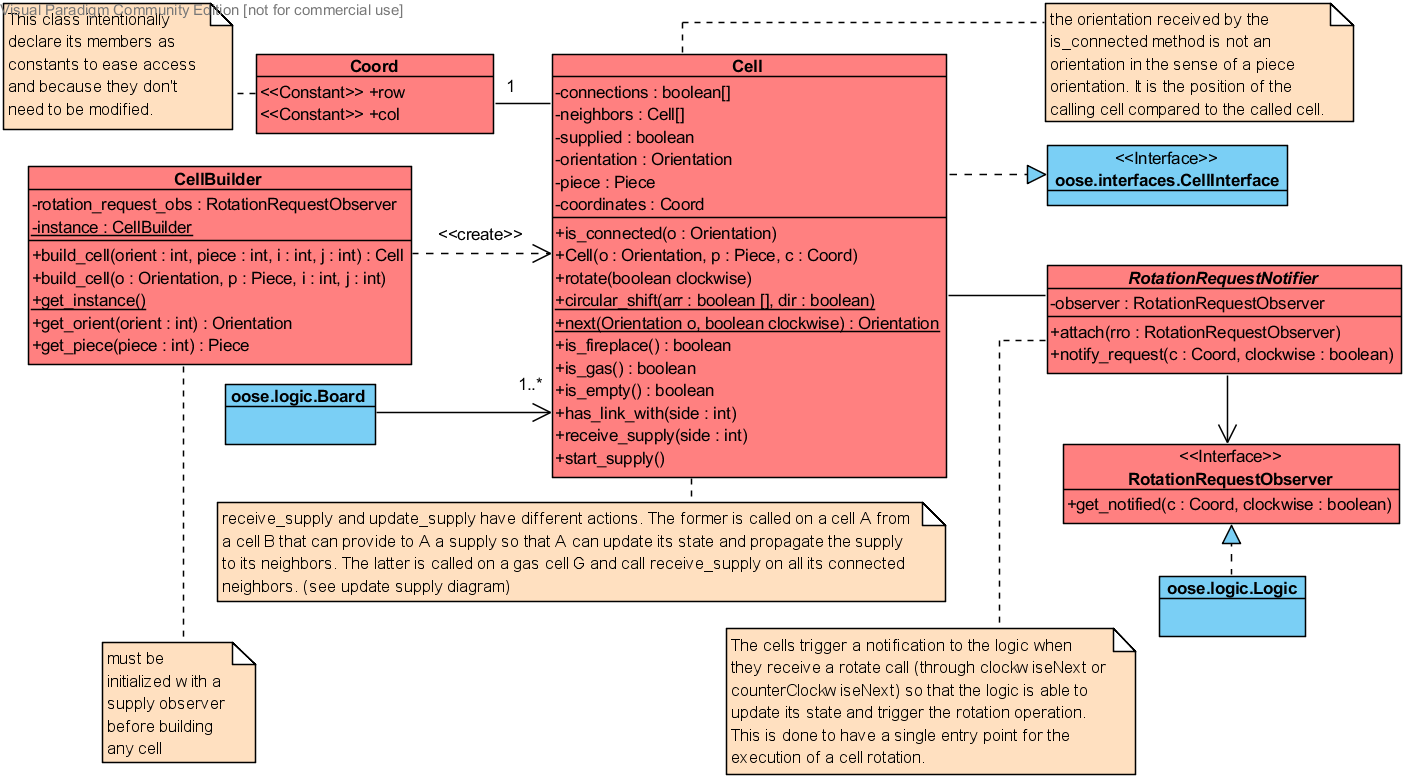
\includegraphics[angle=90,scale=1]{cells.png}
	\caption{Cells}
	\label{fig:cells}
\end{figure}
\subsection{Sequence diagrams}
\begin{figure}
	\center
	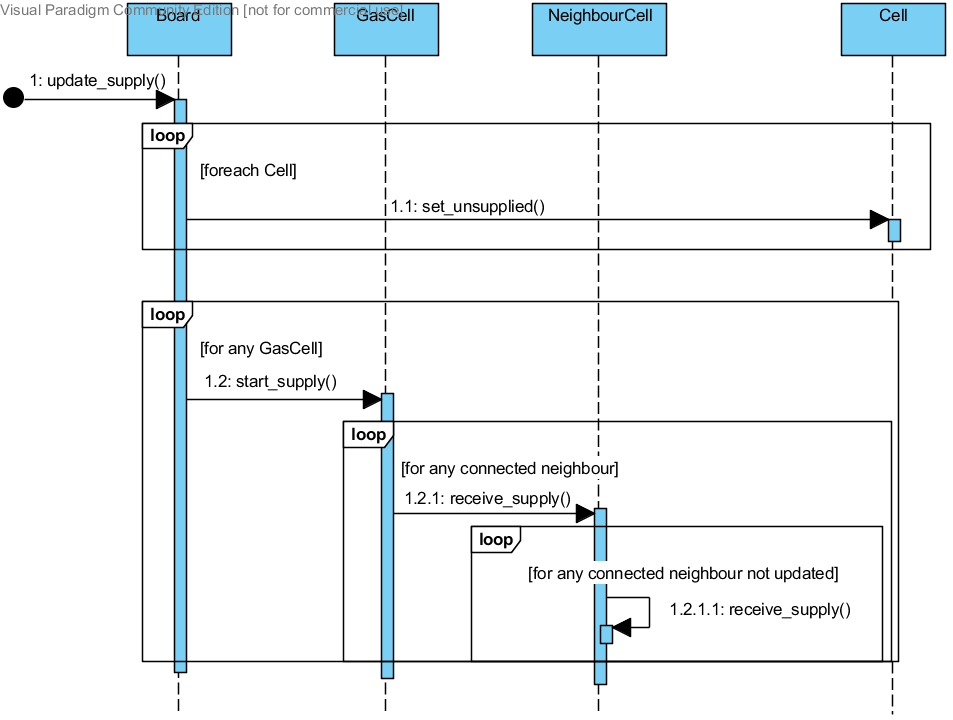
\includegraphics[angle=90,scale=1]{supply_update.png}
	\caption{Supply update}
	\label{fig:sup_update}
\end{figure}
\begin{figure}
	\center
	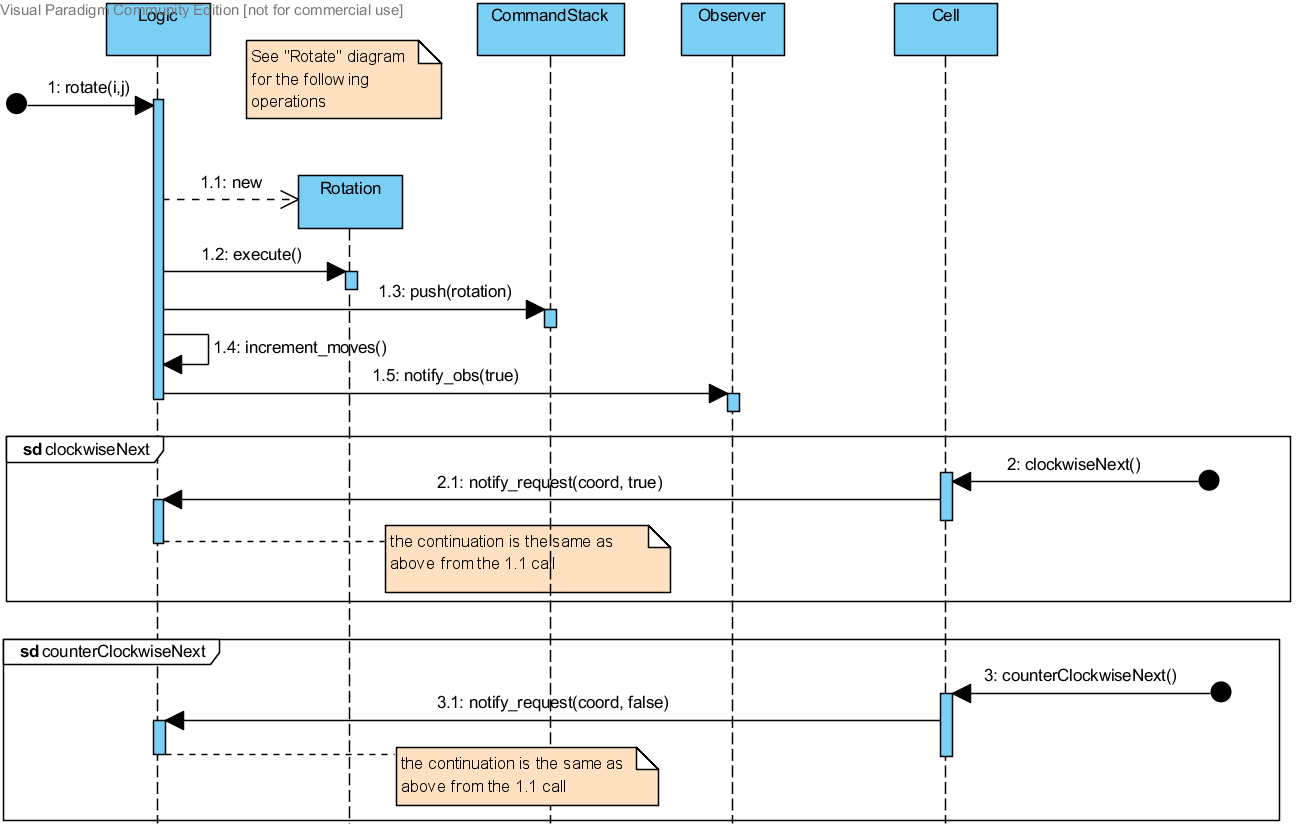
\includegraphics[angle=90,scale=1]{rotation_request.png}
	\caption{Rotation request}
	\label{fig:rot_request}
\end{figure}
\begin{figure}
	\center
	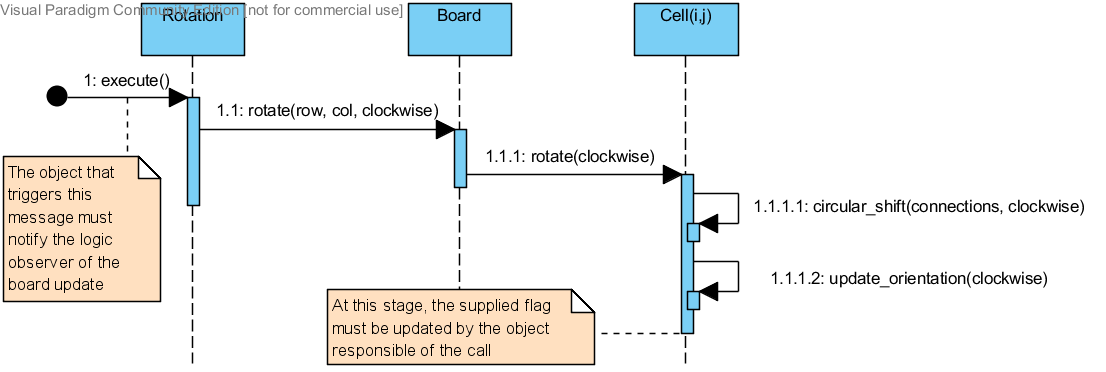
\includegraphics[angle=90,scale=1]{rotation.png}
	\caption{Rotation}
	\label{fig:rotation}
\end{figure}
\begin{figure}
	\center
	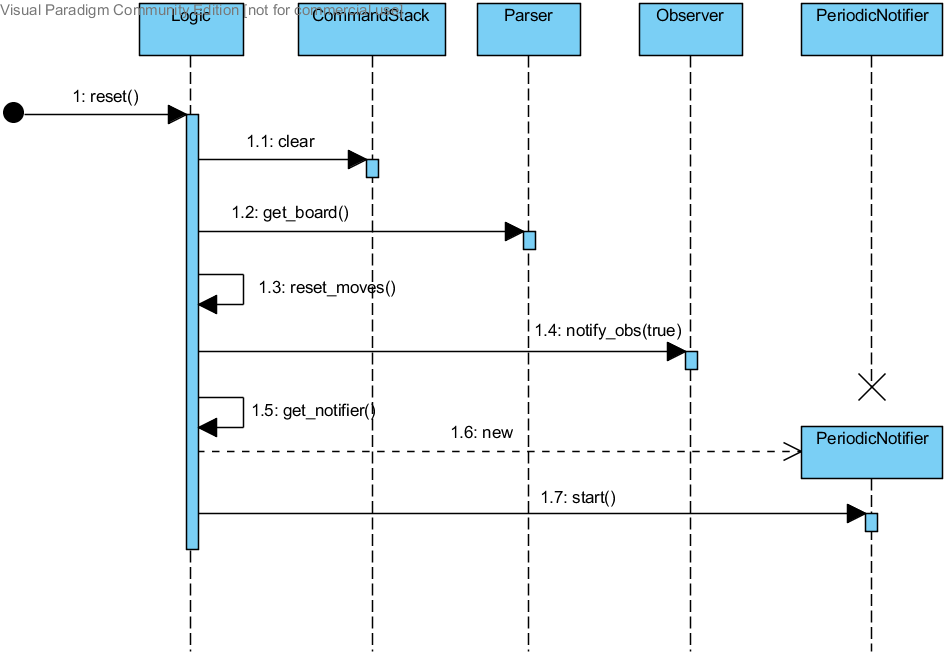
\includegraphics[angle=90,scale=1]{reset.png}
	\caption{Reset}
	\label{fig:reset}
\end{figure}
\begin{figure}
	\center
	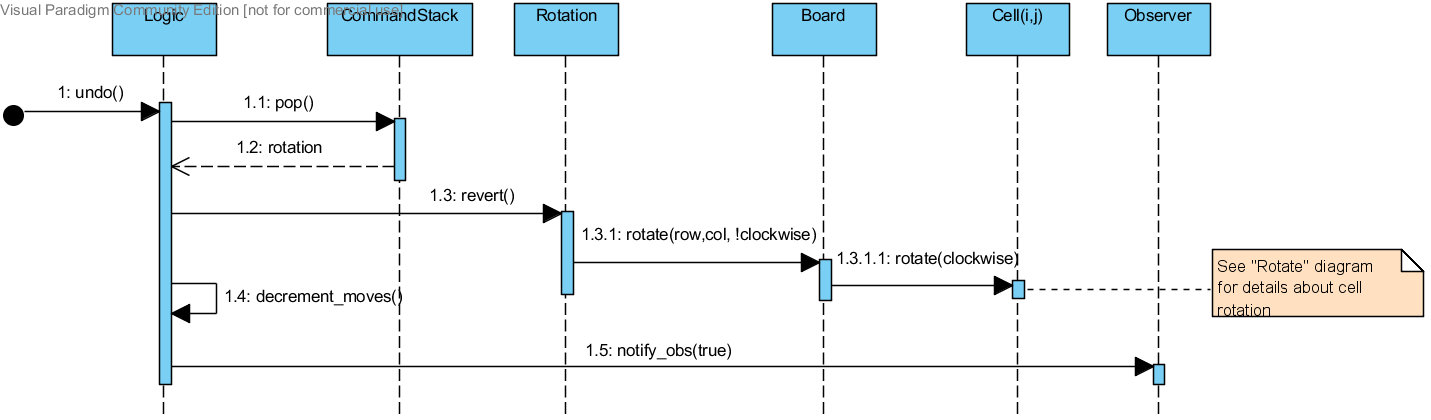
\includegraphics[angle=90,scale=1]{undo.png}
	\caption{Undo}
	\label{fig:undo}
\end{figure}
\end{document}
